\chapter{Voltage peak transducer}
\section{Theory and related work} \label{sec:literature_voltage_peak_transducer}
The design chosen for this voltage peak transducer utilized a resistor divider network as well as a half wave precision rectifier. A resistor divider network is a series connection of two resistors and is used to decrease the magnitude of an input voltage to an acceptable level so that it can be measured. An important element in the design of this circuit is to minimise any current flow in the resistors, thus large resistor values must be chosen. A precision rectifier is an operational amplifier circuit configuration that allows a rectifier circuit to behave like an ideal diode and rectifier, an advantage of this circuit is that it allows us to rectify voltages smaller than the forward voltage of the diode.

\section{Design} \label{sec:design_voltage_peak_transducer}
%In this section, you need to capture your design, which should include the following: 
%\begin{itemize}
%  \item Design rationale, i.e. what your thinking was behind the design
%  \item Design calculations, for example to determine resistor values and capacitor values, or to check for allowed voltage and current ranges and levels. 
%  \item Circuit diagram.
%\end{itemize}
The first step in this design was to design a circuit that would step the fairly large \SI{18}{VAC} input down to a analogue voltage usable by the operational amplifier circuitry, for simplicity a simple resistor divider network was chosen. It was found that the largest differential mode input to the TLC2272 was equal to $V_{DD}=\SI{5}{V}$ and the absolute minimum input was found as $V_{EE}-\SI{0.3}{V}=\SI{-5.3}{V}$ \ref{yourmom}. It was also found that each TLC2272 chip required roughly \SI{2.4}{\milli A} at room temperature given a supply voltage $V_{DD}=\SI{5}{V}$. Referring to Figure \ref{fig:system_diagram} we can see that this design required two of these chips, and thus it was decided that for the voltage transducer a single supply would be used as to not exceed the limitations of the negative voltage supply rail specified in the first report. 
Given this information a 1N4007 diode was placed in series with the voltage divider as to not exceed the new maximum negative differential mode input, $V_{EE}-\SI{0.3}{V}=\SI{-0.3}{V}$. Choosing an absolute maximum input voltage of \SI{24}{VAC}, and compensating for the forward voltage of the diode, the input to the resistor divider network was found to be $V_{in}=\SI{23.3}{VAC}$. To keep power losses to a minimum $R_{2}=\SI{10}{\kilo \Omega}$ was chosen, The value of $R_{1}$ can be found by using Equation \ref{eq:voltagedivider}. After rearranging the terms and substituting for the values, we find that $R_{1}=\SI{56.6}{\kilo \Omega}$, which is very close to the chosen standard resistor value of $\SI{56}{\kilo \Omega}$.\newline
\begin{align}
   V_{DD}=\frac{R_2}{R_1+R_2}V_{in}
   \label{eq:voltagedivider}
\end{align}
The peak detection circuit chosen for this design was a simple precision rectifier as can be seen in Figure \ref{fig:voltagepeakdetector.pdf}. To minimise any power losses in the operational amplifier, a resistor $R_3=\SI{10}{\kilo \Omega}$ was placed at its positive input pin. Since the Arduino's pins work with a voltage level of $\SI{5}{V}$ and the resistor divider network outputs a voltage of up to $\SI{5}{V}$ we require the operational amplifier to have a gain of 1, thus a feedback resistor $R_4$ with a resistance equal to that of $R_3$ had to be placed between the negative input pin and the anode of the diode.
The final part of the peak detection circuit requires a capacitor and resistor with an adequate RC constant as to maintain the desired peak voltage to be measured by the Arduino. A chosen ripple voltage of no more than $\SI{5}{\milli V}$ was chosen for this design and the required capacitor could then be found by applying Equation \ref{eq:ripplevoltage}. With a maximum input voltage $V_{m}=\SI{5}{V}$, a frequency of \SI{50}{Hz}, the internal resistance of the Arduino's pins $R=\SI{1}{M\Omega}$ we can see that the desired capacitor value needs to be equals to $C=\SI{20}{\micro F}$.\newline
\begin{align}
  V_{r} = \frac{V_{m}}{fRC} 
   \label{eq:ripplevoltage}
\end{align}
Given the specification of a maximum input voltage of $\SI{24}{VAC}$ corresponding to a voltage of $\SI{5}{VAC}$ and the Arduino having a range of $4095$ bits, it can be calculated that the resolution of the ADC would be $\SI{8.1175}{\milli V}$ per bit, taking the forward voltage of the rectifier diode into consideration. To ensure that the transducer met the design requirement of responding to a $\SI{1}{V}$ change, which corresponds to an output voltage change of $\SI{151.15}{\milli \volt}$, within 1 second, Equation \ref{eq:capacitordischarge} had to be used. Here $V_{c}=\SI{21.627}{V}$, which corresponds to \SI{1}{V} change in input, $V_{s}=\SI{22.627}{V}$, which corresponds to an input of \SI{16}{VAC}. The resistance $R=\SI{1}{\kilo \Omega}$ and the capacitance $C=\SI{1o}{\micro F}$, given these values the time taken 
\begin{align}
  V_{c} = V_{s}e^{\frac{t}{RC}}
   \label{eq:capacitordischarge}
\end{align}
\begin{figure}[h!]
    \centering
    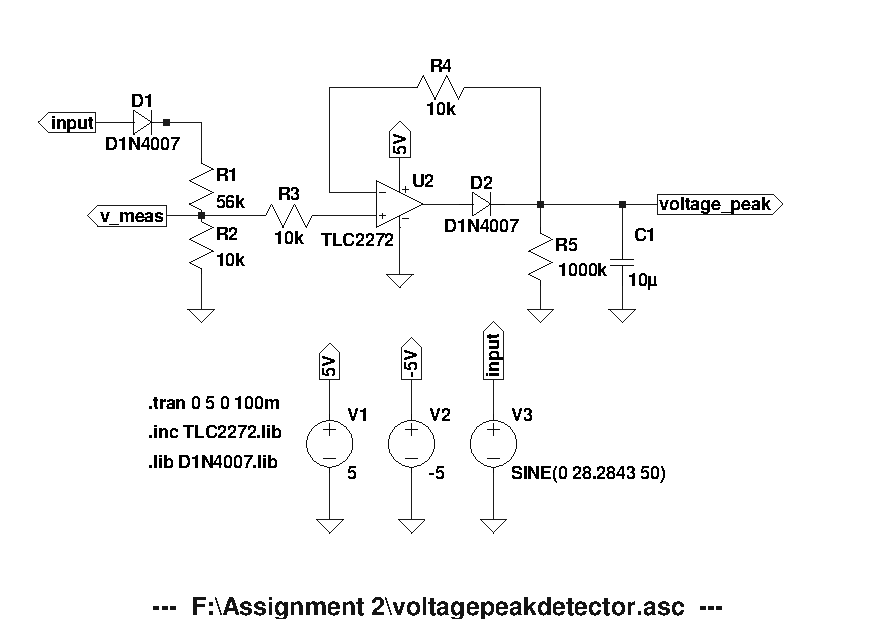
\includegraphics[width = 0.65\linewidth]{Figures/voltagepeakdetector.pdf}
        \caption{Voltage Peak Transducer Diagram}
    \label{fig:voltagepeakdetector.pdf}
\end{figure}


\section{Simulation} \label{sec:simulation_voltage_peak_transducer}
%In this section, you want to demonstrate, by means of simulation results, using the designed circuit, what your circuit is expected to behave. An example is the figure shown in Figure \ref{fig:simulation_results_box} or Subfigure \ref{subfig:AC}. Be absolutely sure that the text and information in your report are readable. 
Firstly the designed voltage transducer was tested given the nominal input voltage of $\SI{18}{VAC}$ and the output can be seen in Figure 

\begin{figure}
 \centering
     \begin{subfigure}[]{0.45\textwidth}
        \centering
         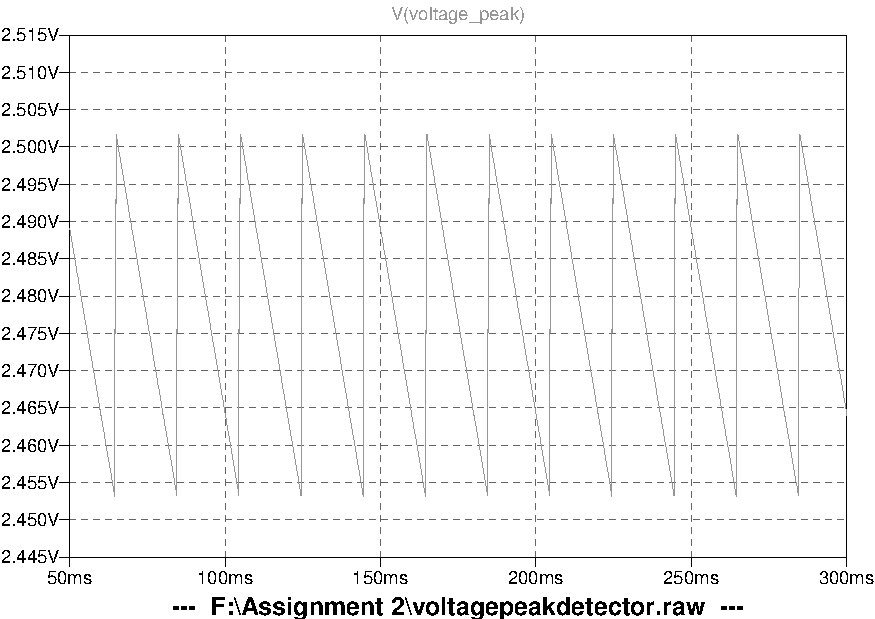
\includegraphics[width=1\linewidth]{./Figures/voltagetransducer12vsim.pdf}
		    \caption{\SI{12}{\volt AC} supply voltage.} \label{subfig:AC}
     \end{subfigure}
      \begin{subfigure}[]{0.45\textwidth}
              \centering
  		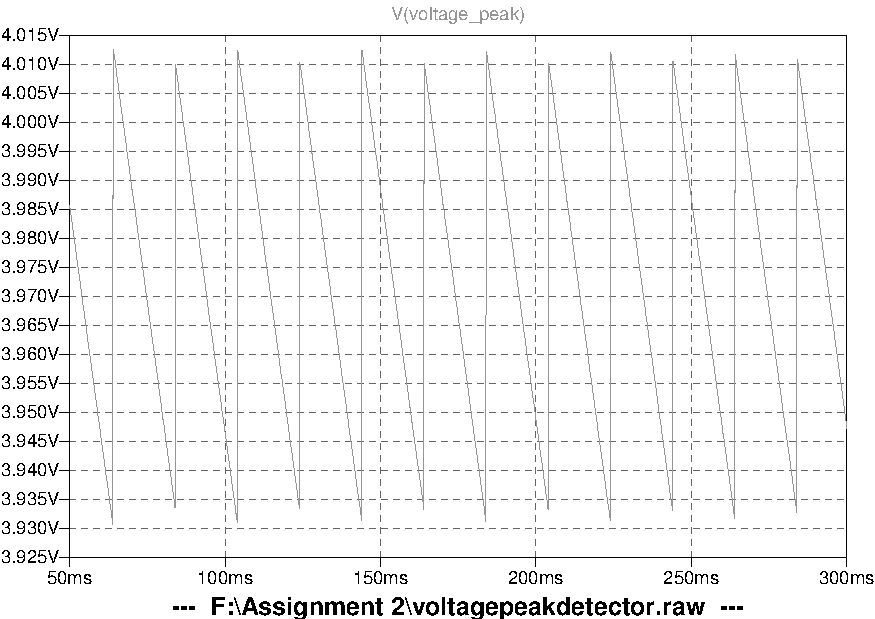
\includegraphics[width=1\linewidth]{./Figures/voltagetransducer20vsim.pdf}
		    \caption{\SI{20}{\volt AC} supply voltage.}
     \end{subfigure}
     \begin{subfigure}[]{0.45\textwidth} 
             \centering
         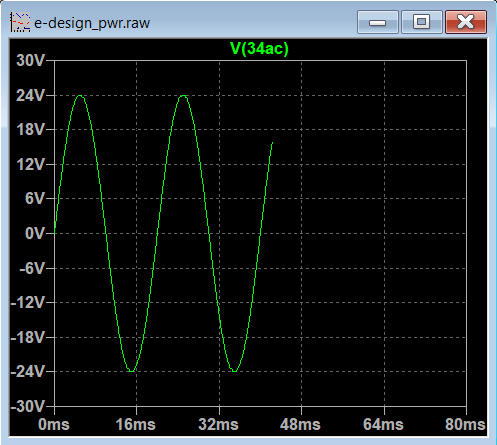
\includegraphics[width=1.\linewidth]{./Figures/Screengrab.png}
		\caption{It is OK to use a screengrab if you are technologically challenged, my mum is too. }
     \end{subfigure}
     \begin{subfigure}[]{0.45\textwidth}
             \centering
  		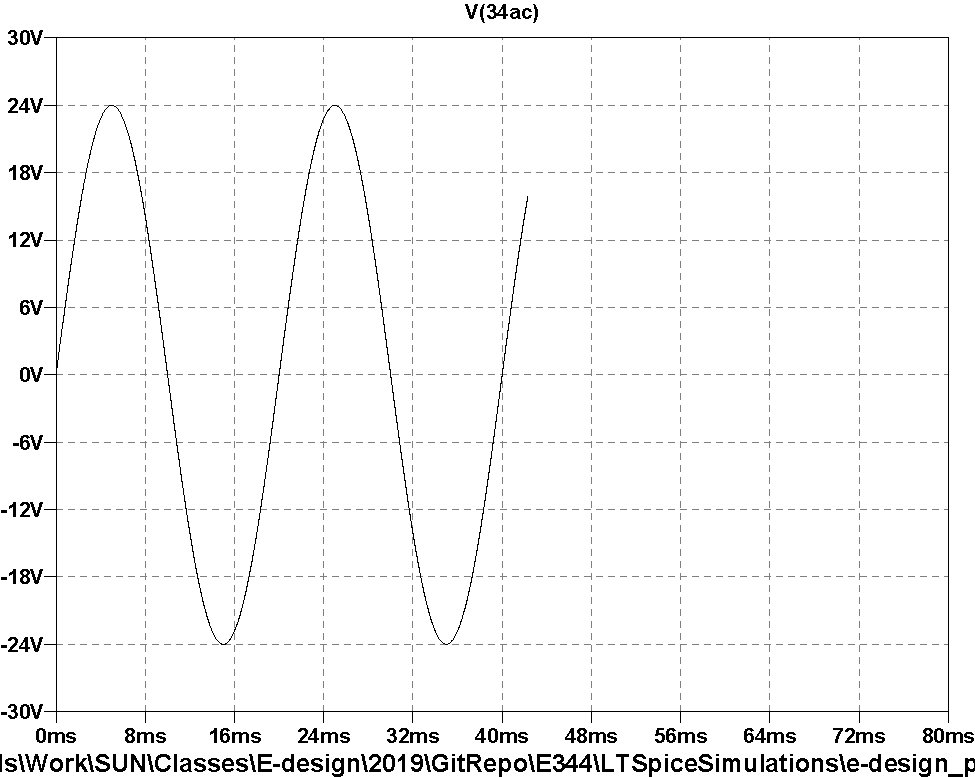
\includegraphics[width=1.0\linewidth]{./Figures/e-design_pwr_ac.pdf}
		   \caption{Say something, I'm giving up on you. }
     \end{subfigure}
   \caption[I am the short caption for the list of figures]{Energy and temperature results of the different control strategies represented as distributions for all water heaters. (a) depicts  electrical energy used per EWH per day, (b) depicts thermal energy drawn per EWH per day, (c) depicts outlet temperatures during usage events, (d) depicts thermal losses per EWH per day. }
    \label{fig:simulation_results_box}
 \end{figure}

\section{Measurements} \label{sec:measurement_voltage_peak_transducer}

In this secion, you must present your measured results. You can use screengrabs or photos of the oscilloscope, or download the CSVs and plot them as PDFs using Matlab, Excel or similar. 
